\documentclass[11pt,compress,t,notes=noshow, xcolor=table]{beamer}
\documentclass[11pt,compress,t,notes=noshow, xcolor=table]{beamer}
\usepackage[]{graphicx}\usepackage[]{color}
% maxwidth is the original width if it is less than linewidth
% otherwise use linewidth (to make sure the graphics do not exceed the margin)
\makeatletter
\def\maxwidth{ %
  \ifdim\Gin@nat@width>\linewidth
    \linewidth
  \else
    \Gin@nat@width
  \fi
}
\makeatother

\definecolor{fgcolor}{rgb}{0.345, 0.345, 0.345}
\newcommand{\hlnum}[1]{\textcolor[rgb]{0.686,0.059,0.569}{#1}}%
\newcommand{\hlstr}[1]{\textcolor[rgb]{0.192,0.494,0.8}{#1}}%
\newcommand{\hlcom}[1]{\textcolor[rgb]{0.678,0.584,0.686}{\textit{#1}}}%
\newcommand{\hlopt}[1]{\textcolor[rgb]{0,0,0}{#1}}%
\newcommand{\hlstd}[1]{\textcolor[rgb]{0.345,0.345,0.345}{#1}}%
\newcommand{\hlkwa}[1]{\textcolor[rgb]{0.161,0.373,0.58}{\textbf{#1}}}%
\newcommand{\hlkwb}[1]{\textcolor[rgb]{0.69,0.353,0.396}{#1}}%
\newcommand{\hlkwc}[1]{\textcolor[rgb]{0.333,0.667,0.333}{#1}}%
\newcommand{\hlkwd}[1]{\textcolor[rgb]{0.737,0.353,0.396}{\textbf{#1}}}%
\let\hlipl\hlkwb

\usepackage{framed}
\makeatletter
\newenvironment{kframe}{%
 \def\at@end@of@kframe{}%
 \ifinner\ifhmode%
  \def\at@end@of@kframe{\end{minipage}}%
  \begin{minipage}{\columnwidth}%
 \fi\fi%
 \def\FrameCommand##1{\hskip\@totalleftmargin \hskip-\fboxsep
 \colorbox{shadecolor}{##1}\hskip-\fboxsep
     % There is no \\@totalrightmargin, so:
     \hskip-\linewidth \hskip-\@totalleftmargin \hskip\columnwidth}%
 \MakeFramed {\advance\hsize-\width
   \@totalleftmargin\z@ \linewidth\hsize
   \@setminipage}}%
 {\par\unskip\endMakeFramed%
 \at@end@of@kframe}
\makeatother

\definecolor{shadecolor}{rgb}{.97, .97, .97}
\definecolor{messagecolor}{rgb}{0, 0, 0}
\definecolor{warningcolor}{rgb}{1, 0, 1}
\definecolor{errorcolor}{rgb}{1, 0, 0}
\newenvironment{knitrout}{}{} % an empty environment to be redefined in TeX

\usepackage{alltt}
\newcommand{\SweaveOpts}[1]{}  % do not interfere with LaTeX
\newcommand{\SweaveInput}[1]{} % because they are not real TeX commands
\newcommand{\Sexpr}[1]{}       % will only be parsed by R
\newcommand{\xmark}{\ding{55}}%


\usepackage[english]{babel}
\usepackage[utf8]{inputenc}

\usepackage{dsfont}
\usepackage{verbatim}
\usepackage{amsmath}
\usepackage{amsfonts}
\usepackage{amssymb}
\usepackage{bm}
\usepackage{csquotes}
\usepackage{multirow}
\usepackage{longtable}
\usepackage{booktabs}
\usepackage{enumerate}
\usepackage[absolute,overlay]{textpos}
\usepackage{psfrag}
\usepackage{algorithm}
\usepackage{algpseudocode}
\usepackage{eqnarray}
\usepackage{arydshln}
\usepackage{tabularx}
\usepackage{placeins}
\usepackage{tikz}
\usepackage{setspace}
\usepackage{colortbl}
\usepackage{mathtools}
\usepackage{wrapfig}
\usepackage{bm}
\usepackage{amsmath}
\usepackage{pifont}

\usetikzlibrary{shapes,arrows,automata,positioning,calc,chains,trees, shadows}
\tikzset{
  %Define standard arrow tip
  >=stealth',
  %Define style for boxes
  punkt/.style={
    rectangle,
    rounded corners,
    draw=black, very thick,
    text width=6.5em,
    minimum height=2em,
    text centered},
  % Define arrow style
  pil/.style={
    ->,
    thick,
    shorten <=2pt,
    shorten >=2pt,}
}

\usepackage{subfig}

% Defines macros and environments
\usepackage{../../style/lmu-lecture}


\let\code=\texttt
\let\proglang=\textsf

\setkeys{Gin}{width=0.9\textwidth}

\setbeamertemplate{frametitle}{\expandafter\uppercase\expandafter\insertframetitle}

% This file is included in slides and exercises

% Rarely used fontstyle for R packages, used only in 
% - forests/slides-forests-benchmark.tex
% - exercises/single-exercises/methods_l_1.Rnw
% - slides/cart/attic/slides_extra_trees.Rnw
\newcommand{\pkg}[1]{{\fontseries{b}\selectfont #1}}

% Spacing helpers, used often (mostly in exercises for \dlz)
\newcommand{\lz}{\vspace{0.5cm}} % vertical space (used often in slides)
\newcommand{\dlz}{\vspace{1cm}}  % double vertical space (used often in exercises, never in slides)
\newcommand{\oneliner}[1] % Oneliner for important statements, used e.g. in iml, algods
{\begin{block}{}\begin{center}\begin{Large}#1\end{Large}\end{center}\end{block}}

% Don't know if this is used or needed, remove?
% textcolor that works in mathmode
% https://tex.stackexchange.com/a/261480
% Used e.g. in forests/slides-forests-bagging.tex
% [...] \textcolor{blue}{\tfrac{1}{M}\sum^M_{m} [...]
% \makeatletter
% \renewcommand*{\@textcolor}[3]{%
%   \protect\leavevmode
%   \begingroup
%     \color#1{#2}#3%
%   \endgroup
% }
% \makeatother






% latex-math includes as needed
% dependencies: amsmath, amssymb, dsfont
% math spaces
\ifdefined\N
\renewcommand{\N}{\mathds{N}} % N, naturals
\else \newcommand{\N}{\mathds{N}} \fi
\newcommand{\Z}{\mathds{Z}} % Z, integers
\newcommand{\Q}{\mathds{Q}} % Q, rationals
\newcommand{\R}{\mathds{R}} % R, reals
\ifdefined\C
\renewcommand{\C}{\mathds{C}} % C, complex
\else \newcommand{\C}{\mathds{C}} \fi
\newcommand{\continuous}{\mathcal{C}} % C, space of continuous functions
\newcommand{\M}{\mathcal{M}} % machine numbers
\newcommand{\epsm}{\epsilon_m} % maximum error

% counting / finite sets
\newcommand{\setzo}{\{0, 1\}} % set 0, 1
\newcommand{\setmp}{\{-1, +1\}} % set -1, 1
\newcommand{\unitint}{[0, 1]} % unit interval

% basic math stuff
\newcommand{\xt}{\tilde x} % x tilde
\newcommand{\argmin}{\mathop{\mathrm{arg\,min}}} % argmin
\newcommand{\argmax}{\mathop{\mathrm{arg\,max}}} % argmax
\newcommand{\argminlim}{\argmin\limits} % argmin with limits
\newcommand{\argmaxlim}{\argmax\limits} % argmax with limits
\newcommand{\sign}{\operatorname{sign}} % sign, signum
\newcommand{\I}{\mathbb{I}} % I, indicator
\newcommand{\order}{\mathcal{O}} % O, order
\newcommand{\bigO}{\mathcal{O}} % Big-O Landau
\newcommand{\littleo}{{o}} % Little-o Landau
\newcommand{\pd}[2]{\frac{\partial{#1}}{\partial #2}} % partial derivative
\newcommand{\floorlr}[1]{\left\lfloor #1 \right\rfloor} % floor
\newcommand{\ceillr}[1]{\left\lceil #1 \right\rceil} % ceiling
\newcommand{\indep}{\perp \!\!\! \perp} % independence symbol

% sums and products
\newcommand{\sumin}{\sum\limits_{i=1}^n} % summation from i=1 to n
\newcommand{\sumim}{\sum\limits_{i=1}^m} % summation from i=1 to m
\newcommand{\sumjn}{\sum\limits_{j=1}^n} % summation from j=1 to p
\newcommand{\sumjp}{\sum\limits_{j=1}^p} % summation from j=1 to p
\newcommand{\sumik}{\sum\limits_{i=1}^k} % summation from i=1 to k
\newcommand{\sumkg}{\sum\limits_{k=1}^g} % summation from k=1 to g
\newcommand{\sumjg}{\sum\limits_{j=1}^g} % summation from j=1 to g
\newcommand{\summM}{\sum\limits_{m=1}^M} % summation from m=1 to M
\newcommand{\meanin}{\frac{1}{n} \sum\limits_{i=1}^n} % mean from i=1 to n
\newcommand{\meanim}{\frac{1}{m} \sum\limits_{i=1}^m} % mean from i=1 to n
\newcommand{\meankg}{\frac{1}{g} \sum\limits_{k=1}^g} % mean from k=1 to g
\newcommand{\meanmM}{\frac{1}{M} \sum\limits_{m=1}^M} % mean from m=1 to M
\newcommand{\prodin}{\prod\limits_{i=1}^n} % product from i=1 to n
\newcommand{\prodkg}{\prod\limits_{k=1}^g} % product from k=1 to g
\newcommand{\prodjp}{\prod\limits_{j=1}^p} % product from j=1 to p

% linear algebra
\newcommand{\one}{\bm{1}} % 1, unitvector
\newcommand{\zero}{\mathbf{0}} % 0-vector
\newcommand{\id}{\bm{I}} % I, identity
\newcommand{\diag}{\operatorname{diag}} % diag, diagonal
\newcommand{\trace}{\operatorname{tr}} % tr, trace
\newcommand{\spn}{\operatorname{span}} % span
\newcommand{\scp}[2]{\left\langle #1, #2 \right\rangle} % <.,.>, scalarproduct
\newcommand{\mat}[1]{\begin{pmatrix} #1 \end{pmatrix}} % short pmatrix command
\newcommand{\Amat}{\mathbf{A}} % matrix A
\newcommand{\Deltab}{\mathbf{\Delta}} % error term for vectors

% basic probability + stats
\renewcommand{\P}{\mathds{P}} % P, probability
\newcommand{\E}{\mathds{E}} % E, expectation
\newcommand{\var}{\mathsf{Var}} % Var, variance
\newcommand{\cov}{\mathsf{Cov}} % Cov, covariance
\newcommand{\corr}{\mathsf{Corr}} % Corr, correlation
\newcommand{\normal}{\mathcal{N}} % N of the normal distribution
\newcommand{\iid}{\overset{i.i.d}{\sim}} % dist with i.i.d superscript
\newcommand{\distas}[1]{\overset{#1}{\sim}} % ... is distributed as ...

% machine learning
\newcommand{\Xspace}{\mathcal{X}} % X, input space
\newcommand{\Yspace}{\mathcal{Y}} % Y, output space
\newcommand{\Zspace}{\mathcal{Z}} % Z, space of sampled datapoints
\newcommand{\nset}{\{1, \ldots, n\}} % set from 1 to n
\newcommand{\pset}{\{1, \ldots, p\}} % set from 1 to p
\newcommand{\gset}{\{1, \ldots, g\}} % set from 1 to g
\newcommand{\Pxy}{\mathbb{P}_{xy}} % P_xy
\newcommand{\Exy}{\mathbb{E}_{xy}} % E_xy: Expectation over random variables xy
\newcommand{\xv}{\mathbf{x}} % vector x (bold)
\newcommand{\xtil}{\tilde{\mathbf{x}}} % vector x-tilde (bold)
\newcommand{\yv}{\mathbf{y}} % vector y (bold)
\newcommand{\xy}{(\xv, y)} % observation (x, y)
\newcommand{\xvec}{\left(x_1, \ldots, x_p\right)^\top} % (x1, ..., xp)
\newcommand{\Xmat}{\mathbf{X}} % Design matrix
\newcommand{\allDatasets}{\mathds{D}} % The set of all datasets
\newcommand{\allDatasetsn}{\mathds{D}_n}  % The set of all datasets of size n
\newcommand{\D}{\mathcal{D}} % D, data
\newcommand{\Dn}{\D_n} % D_n, data of size n
\newcommand{\Dtrain}{\mathcal{D}_{\text{train}}} % D_train, training set
\newcommand{\Dtest}{\mathcal{D}_{\text{test}}} % D_test, test set
\newcommand{\xyi}[1][i]{\left(\xv^{(#1)}, y^{(#1)}\right)} % (x^i, y^i), i-th observation
\newcommand{\Dset}{\left( \xyi[1], \ldots, \xyi[n]\right)} % {(x1,y1)), ..., (xn,yn)}, data
\newcommand{\defAllDatasetsn}{(\Xspace \times \Yspace)^n} % Def. of the set of all datasets of size n
\newcommand{\defAllDatasets}{\bigcup_{n \in \N}(\Xspace \times \Yspace)^n} % Def. of the set of all datasets
\newcommand{\xdat}{\left\{ \xv^{(1)}, \ldots, \xv^{(n)}\right\}} % {x1, ..., xn}, input data
\newcommand{\ydat}{\left\{ \yv^{(1)}, \ldots, \yv^{(n)}\right\}} % {y1, ..., yn}, input data
\newcommand{\yvec}{\left(y^{(1)}, \hdots, y^{(n)}\right)^\top} % (y1, ..., yn), vector of outcomes
\newcommand{\greekxi}{\xi} % Greek letter xi
\renewcommand{\xi}[1][i]{\xv^{(#1)}} % x^i, i-th observed value of x
\newcommand{\yi}[1][i]{y^{(#1)}} % y^i, i-th observed value of y
\newcommand{\xivec}{\left(x^{(i)}_1, \ldots, x^{(i)}_p\right)^\top} % (x1^i, ..., xp^i), i-th observation vector
\newcommand{\xj}{\xv_j} % x_j, j-th feature
\newcommand{\xjvec}{\left(x^{(1)}_j, \ldots, x^{(n)}_j\right)^\top} % (x^1_j, ..., x^n_j), j-th feature vector
\newcommand{\phiv}{\mathbf{\phi}} % Basis transformation function phi
\newcommand{\phixi}{\mathbf{\phi}^{(i)}} % Basis transformation of xi: phi^i := phi(xi)

%%%%%% ml - models general
\newcommand{\lamv}{\bm{\lambda}} % lambda vector, hyperconfiguration vector
\newcommand{\Lam}{\bm{\Lambda}}	 % Lambda, space of all hpos
% Inducer / Inducing algorithm
\newcommand{\preimageInducer}{\left(\defAllDatasets\right)\times\Lam} % Set of all datasets times the hyperparameter space
\newcommand{\preimageInducerShort}{\allDatasets\times\Lam} % Set of all datasets times the hyperparameter space
% Inducer / Inducing algorithm
\newcommand{\ind}{\mathcal{I}} % Inducer, inducing algorithm, learning algorithm

% continuous prediction function f
\newcommand{\ftrue}{f_{\text{true}}}  % True underlying function (if a statistical model is assumed)
\newcommand{\ftruex}{\ftrue(\xv)} % True underlying function (if a statistical model is assumed)
\newcommand{\fx}{f(\xv)} % f(x), continuous prediction function
\newcommand{\fdomains}{f: \Xspace \rightarrow \R^g} % f with domain and co-domain
\newcommand{\Hspace}{\mathcal{H}} % hypothesis space where f is from
\newcommand{\fbayes}{f^{\ast}} % Bayes-optimal model
\newcommand{\fxbayes}{f^{\ast}(\xv)} % Bayes-optimal model
\newcommand{\fkx}[1][k]{f_{#1}(\xv)} % f_j(x), discriminant component function
\newcommand{\fh}{\hat{f}} % f hat, estimated prediction function
\newcommand{\fxh}{\fh(\xv)} % fhat(x)
\newcommand{\fxt}{f(\xv ~|~ \thetav)} % f(x | theta)
\newcommand{\fxi}{f\left(\xv^{(i)}\right)} % f(x^(i))
\newcommand{\fxih}{\hat{f}\left(\xv^{(i)}\right)} % f(x^(i))
\newcommand{\fxit}{f\left(\xv^{(i)} ~|~ \thetav\right)} % f(x^(i) | theta)
\newcommand{\fhD}{\fh_{\D}} % fhat_D, estimate of f based on D
\newcommand{\fhDtrain}{\fh_{\Dtrain}} % fhat_Dtrain, estimate of f based on D
\newcommand{\fhDnlam}{\fh_{\Dn, \lamv}} %model learned on Dn with hp lambda
\newcommand{\fhDlam}{\fh_{\D, \lamv}} %model learned on D with hp lambda
\newcommand{\fhDnlams}{\fh_{\Dn, \lamv^\ast}} %model learned on Dn with optimal hp lambda
\newcommand{\fhDlams}{\fh_{\D, \lamv^\ast}} %model learned on D with optimal hp lambda

% discrete prediction function h
\newcommand{\hx}{h(\xv)} % h(x), discrete prediction function
\newcommand{\hh}{\hat{h}} % h hat
\newcommand{\hxh}{\hat{h}(\xv)} % hhat(x)
\newcommand{\hxt}{h(\xv | \thetav)} % h(x | theta)
\newcommand{\hxi}{h\left(\xi\right)} % h(x^(i))
\newcommand{\hxit}{h\left(\xi ~|~ \thetav\right)} % h(x^(i) | theta)
\newcommand{\hbayes}{h^{\ast}} % Bayes-optimal classification model
\newcommand{\hxbayes}{h^{\ast}(\xv)} % Bayes-optimal classification model

% yhat
\newcommand{\yh}{\hat{y}} % yhat for prediction of target
\newcommand{\yih}{\hat{y}^{(i)}} % yhat^(i) for prediction of ith targiet
\newcommand{\resi}{\yi- \yih}

% theta
\newcommand{\thetah}{\hat{\theta}} % theta hat
\newcommand{\thetav}{\bm{\theta}} % theta vector
\newcommand{\thetavh}{\bm{\hat\theta}} % theta vector hat
\newcommand{\thetat}[1][t]{\thetav^{[#1]}} % theta^[t] in optimization
\newcommand{\thetatn}[1][t]{\thetav^{[#1 +1]}} % theta^[t+1] in optimization
\newcommand{\thetahDnlam}{\thetavh_{\Dn, \lamv}} %theta learned on Dn with hp lambda
\newcommand{\thetahDlam}{\thetavh_{\D, \lamv}} %theta learned on D with hp lambda
\newcommand{\mint}{\min_{\thetav \in \Theta}} % min problem theta
\newcommand{\argmint}{\argmin_{\thetav \in \Theta}} % argmin theta

% densities + probabilities
% pdf of x
\newcommand{\pdf}{p} % p
\newcommand{\pdfx}{p(\xv)} % p(x)
\newcommand{\pixt}{\pi(\xv~|~ \thetav)} % pi(x|theta), pdf of x given theta
\newcommand{\pixit}[1][i]{\pi\left(\xi[#1] ~|~ \thetav\right)} % pi(x^i|theta), pdf of x given theta
\newcommand{\pixii}[1][i]{\pi\left(\xi[#1]\right)} % pi(x^i), pdf of i-th x

% pdf of (x, y)
\newcommand{\pdfxy}{p(\xv,y)} % p(x, y)
\newcommand{\pdfxyt}{p(\xv, y ~|~ \thetav)} % p(x, y | theta)
\newcommand{\pdfxyit}{p\left(\xi, \yi ~|~ \thetav\right)} % p(x^(i), y^(i) | theta)

% pdf of x given y
\newcommand{\pdfxyk}[1][k]{p(\xv | y= #1)} % p(x | y = k)
\newcommand{\lpdfxyk}[1][k]{\log p(\xv | y= #1)} % log p(x | y = k)
\newcommand{\pdfxiyk}[1][k]{p\left(\xi | y= #1 \right)} % p(x^i | y = k)

% prior probabilities
\newcommand{\pik}[1][k]{\pi_{#1}} % pi_k, prior
\newcommand{\lpik}[1][k]{\log \pi_{#1}} % log pi_k, log of the prior
\newcommand{\pit}{\pi(\thetav)} % Prior probability of parameter theta

% posterior probabilities
\newcommand{\post}{\P(y = 1 ~|~ \xv)} % P(y = 1 | x), post. prob for y=1
\newcommand{\postk}[1][k]{\P(y = #1 ~|~ \xv)} % P(y = k | y), post. prob for y=k
\newcommand{\pidomains}{\pi: \Xspace \rightarrow \unitint} % pi with domain and co-domain
\newcommand{\pibayes}{\pi^{\ast}} % Bayes-optimal classification model
\newcommand{\pixbayes}{\pi^{\ast}(\xv)} % Bayes-optimal classification model
\newcommand{\pix}{\pi(\xv)} % pi(x), P(y = 1 | x)
\newcommand{\piv}{\bm{\pi}} % pi, bold, as vector
\newcommand{\pikx}[1][k]{\pi_{#1}(\xv)} % pi_k(x), P(y = k | x)
\newcommand{\pikxt}[1][k]{\pi_{#1}(\xv ~|~ \thetav)} % pi_k(x | theta), P(y = k | x, theta)
\newcommand{\pixh}{\hat \pi(\xv)} % pi(x) hat, P(y = 1 | x) hat
\newcommand{\pikxh}[1][k]{\hat \pi_{#1}(\xv)} % pi_k(x) hat, P(y = k | x) hat
\newcommand{\pixih}{\hat \pi(\xi)} % pi(x^(i)) with hat
\newcommand{\pikxih}[1][k]{\hat \pi_{#1}(\xi)} % pi_k(x^(i)) with hat
\newcommand{\pdfygxt}{p(y ~|~\xv, \thetav)} % p(y | x, theta)
\newcommand{\pdfyigxit}{p\left(\yi ~|~\xi, \thetav\right)} % p(y^i |x^i, theta)
\newcommand{\lpdfygxt}{\log \pdfygxt } % log p(y | x, theta)
\newcommand{\lpdfyigxit}{\log \pdfyigxit} % log p(y^i |x^i, theta)

% probababilistic
\newcommand{\bayesrulek}[1][k]{\frac{\P(\xv | y= #1) \P(y= #1)}{\P(\xv)}} % Bayes rule
\newcommand{\muk}{\bm{\mu_k}} % mean vector of class-k Gaussian (discr analysis)

% residual and margin
\newcommand{\eps}{\epsilon} % residual, stochastic
\newcommand{\epsv}{\bm{\epsilon}} % residual, stochastic, as vector
\newcommand{\epsi}{\epsilon^{(i)}} % epsilon^i, residual, stochastic
\newcommand{\epsh}{\hat{\epsilon}} % residual, estimated
\newcommand{\epsvh}{\hat{\epsv}} % residual, estimated, vector
\newcommand{\yf}{y \fx} % y f(x), margin
\newcommand{\yfi}{\yi \fxi} % y^i f(x^i), margin
\newcommand{\Sigmah}{\hat \Sigma} % estimated covariance matrix
\newcommand{\Sigmahj}{\hat \Sigma_j} % estimated covariance matrix for the j-th class

% ml - loss, risk, likelihood
\newcommand{\Lyf}{L\left(y, f\right)} % L(y, f), loss function
\newcommand{\Lypi}{L\left(y, \pi\right)} % L(y, pi), loss function
\newcommand{\Lxy}{L\left(y, \fx\right)} % L(y, f(x)), loss function
\newcommand{\Lxyi}{L\left(\yi, \fxi\right)} % loss of observation
\newcommand{\Lxyt}{L\left(y, \fxt\right)} % loss with f parameterized
\newcommand{\Lxyit}{L\left(\yi, \fxit\right)} % loss of observation with f parameterized
\newcommand{\Lxym}{L\left(\yi, f\left(\bm{\tilde{x}}^{(i)} ~|~ \thetav\right)\right)} % loss of observation with f parameterized
\newcommand{\Lpixy}{L\left(y, \pix\right)} % loss in classification
\newcommand{\Lpiy}{L\left(y, \pi\right)} % loss in classification
\newcommand{\Lpiv}{L\left(y, \piv\right)} % loss in classification
\newcommand{\Lpixyi}{L\left(\yi, \pixii\right)} % loss of observation in classification
\newcommand{\Lpixyt}{L\left(y, \pixt\right)} % loss with pi parameterized
\newcommand{\Lpixyit}{L\left(\yi, \pixit\right)} % loss of observation with pi parameterized
\newcommand{\Lhy}{L\left(y, h\right)} % L(y, h), loss function on discrete classes
\newcommand{\Lhxy}{L\left(y, \hx\right)} % L(y, h(x)), loss function on discrete classes
\newcommand{\Lr}{L\left(r\right)} % L(r), loss defined on residual (reg) / margin (classif)
\newcommand{\lone}{|y - \fx|} % L1 loss
\newcommand{\ltwo}{\left(y - \fx\right)^2} % L2 loss
\newcommand{\lbernoullimp}{\ln(1 + \exp(-y \cdot \fx))} % Bernoulli loss for -1, +1 encoding
\newcommand{\lbernoullizo}{- y \cdot \fx + \log(1 + \exp(\fx))} % Bernoulli loss for 0, 1 encoding
\newcommand{\lcrossent}{- y \log \left(\pix\right) - (1 - y) \log \left(1 - \pix\right)} % cross-entropy loss
\newcommand{\lbrier}{\left(\pix - y \right)^2} % Brier score
\newcommand{\risk}{\mathcal{R}} % R, risk
\newcommand{\riskbayes}{\mathcal{R}^\ast}
\newcommand{\riskf}{\risk(f)} % R(f), risk
\newcommand{\riskdef}{\E_{y|\xv}\left(\Lxy \right)} % risk def (expected loss)
\newcommand{\riskt}{\mathcal{R}(\thetav)} % R(theta), risk
\newcommand{\riske}{\mathcal{R}_{\text{emp}}} % R_emp, empirical risk w/o factor 1 / n
\newcommand{\riskeb}{\bar{\mathcal{R}}_{\text{emp}}} % R_emp, empirical risk w/ factor 1 / n
\newcommand{\riskef}{\riske(f)} % R_emp(f)
\newcommand{\risket}{\mathcal{R}_{\text{emp}}(\thetav)} % R_emp(theta)
\newcommand{\riskr}{\mathcal{R}_{\text{reg}}} % R_reg, regularized risk
\newcommand{\riskrt}{\mathcal{R}_{\text{reg}}(\thetav)} % R_reg(theta)
\newcommand{\riskrf}{\riskr(f)} % R_reg(f)
\newcommand{\riskrth}{\hat{\mathcal{R}}_{\text{reg}}(\thetav)} % hat R_reg(theta)
\newcommand{\risketh}{\hat{\mathcal{R}}_{\text{emp}}(\thetav)} % hat R_emp(theta)
\newcommand{\LL}{\mathcal{L}} % L, likelihood
\newcommand{\LLt}{\mathcal{L}(\thetav)} % L(theta), likelihood
\newcommand{\LLtx}{\mathcal{L}(\thetav | \xv)} % L(theta|x), likelihood
\newcommand{\logl}{\ell} % l, log-likelihood
\newcommand{\loglt}{\logl(\thetav)} % l(theta), log-likelihood
\newcommand{\logltx}{\logl(\thetav | \xv)} % l(theta|x), log-likelihood
\newcommand{\errtrain}{\text{err}_{\text{train}}} % training error
\newcommand{\errtest}{\text{err}_{\text{test}}} % test error
\newcommand{\errexp}{\overline{\text{err}_{\text{test}}}} % avg training error

% lm
\newcommand{\thx}{\thetav^\top \xv} % linear model
\newcommand{\olsest}{(\Xmat^\top \Xmat)^{-1} \Xmat^\top \yv} % OLS estimator in LM


% Lecture title always has to be there
\title{Algorithms and Data Structures}

\begin{document}

\titlemeta{% Chunk title (example: CART, Forests, Boosting, ...), can be empty
Quadrature
}{% Lecture title
Laplace's method
}{% Relative path to title page image: Can be empty but must not start with slides/
}{% Learning goals, wrapped inside itemize environment
  \item Laplace's method
}

%\lecture{CIM1 Statistical Computing}

\begin{vbframe}{Laplace's method}

%<<out.width = '90%', fig.align = "center", echo = FALSE>>=
%# Berechne Posterior für Gamma
%makepost = function(y, shape, scale) {
%        function(x) {
%          dgamma(x, shape = y + shape, scale = 1 / (1 + 1 / scale))
%        }
%}
%@

\textbf{Target:} Approximate integral of function $f$ with the following properties:

\begin{itemize}
\item The mass concentrates on a small area around a center and the function has very rapidly decreasing tails
%approaches $0$ fast for $x \to \pm \infty$ 
("similarity" to the density of a normal distribution)
\item The function we want to integrate is the density of a random variable that is approximately normally distributed
\end{itemize}

% Genauer gesagt fordern wir $f \in \mathcal{L}^2$ (quadratische Integrierbarkeit)
%
% \vspace*{-0.1cm}
%
% $$
% \int f(x)^2 dx < \infty.
% $$


\begin{center}
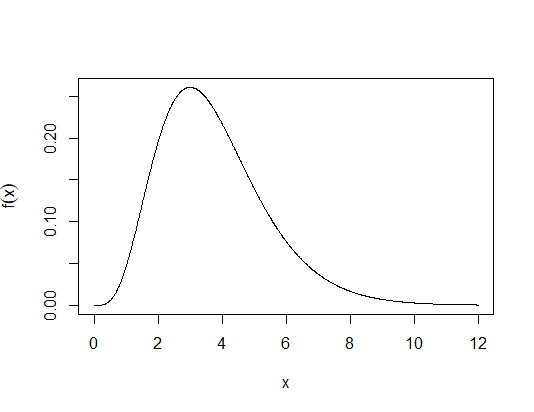
\includegraphics[width =0.5\textwidth]{figure_man/normaldist.png}
\end{center}

%<<out.width = '60%', fig.align = "center", echo = FALSE>>=
%# We're already using the Gamma Posterior distribution here
%# as example function
%# Later we'll explain the example in more detail
%# So far this is just "some" example function
%set.seed(1234)

%y = 2
%prior.shape = 3
%prior.scale = 3

%p = makepost(y, prior.shape, prior.scale)

%pmode = (y + prior.shape - 1) * (1 / (1 + 1 / prior.scale))
%pmean = (y + prior.shape) * (1 / (1 + 1 / prior.scale))

%a = prior.shape
%b = prior.scale

%fhat = deriv3(~ mu^(y + a - 1) * exp(-mu * (1 + 1/b)) / ((1/(1+1/b))^(y+a) * gamma(y + a)), "mu", function.arg = TRUE)

%post.shape = y + prior.shape - 1
%post.scale = 1 / (length(y) + 1 / prior.scale)

%curve(p, 0, 12, n = 1000, xlab = expression(x), ylab = expression(f(x)))
%@



\framebreak
In particular, we assume that $f$

\begin{itemize}
\item Can only be positive
\item Is two times continuously differentiable
\item Has a \textbf{global maximum} at $x_0$
\end{itemize}


%\framebreak
\vspace*{0.1cm}
We could approximate the area underneath the graph of the function with a staircase function and represent the integral with a very simple formula that depends on $f(x_0)$:
\vspace*{-0.1cm}
\begin{footnotesize}
$$
\int f(x)~dx \approx f(x_0) \cdot c
$$

\begin{center}
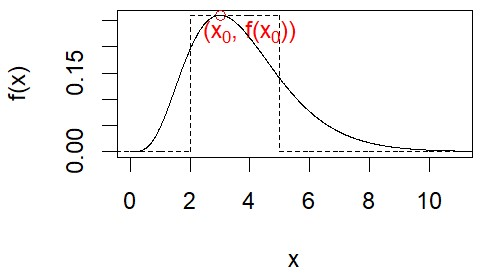
\includegraphics[width =0.5\textwidth]{figure_man/normaldist2.jpg}
\end{center}

%<<out.width = '59%', fig.align = "center", echo = FALSE>>=
%par(cex = 1.5)

%y0 = 0.26 * c(0, 0, rep(1, 3), rep(0, 6))
%sfun = stepfun(1:10, y0, f = 0)
%plot(sfun, main = "", lty = 2, do.points = FALSE)
%points(3, p(3), col = "red")
%text(x = 4, 0.23, expression(paste("(", x[0], ", f(", x[0], "))")), col = "red")
%curve(p, 0, 12, n = 1000, xlab = expression(x), ylab = expression(f(x)), add = TRUE)
%@
\end{footnotesize}

\framebreak

But instead of the step function we would like to choose a function that approximates $f$ \textbf{better} and which has well-known properties.

\lz

\textbf{Idea:} Approximate the integral using the density function of the normal distribution!

\lz

\textbf{How?} We center and scale the density function of the normal distribution such that it approximates $f$ "best possible".

\framebreak

In other words: We determine \textbf{expectation} and \textbf{standard deviation} of a normal distribution such that the corresponding density function fits best possible to the function $f$ we are interested in.

\begin{center}
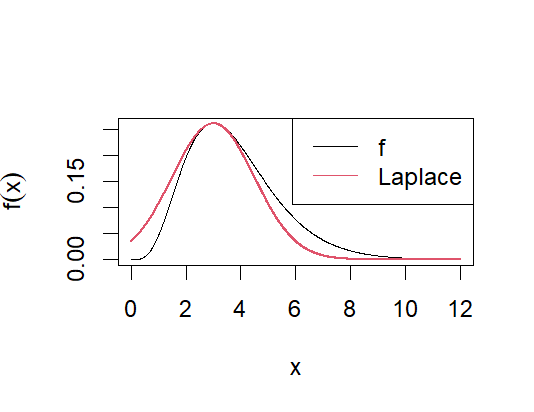
\includegraphics[width =0.7\textwidth]{figure_man/laplace01.png}
\end{center}


\framebreak

\textbf{Mathematical derivation:}

Let there be a function $f$ with a global maximum at $x_0$.

\lz

We define $h(x) := \log f(x)$ as the logarithmized function and rewrite the integral

$$
\int_a^b f(x)~dx = \int_a^b \exp(\underbrace{\log f(x)}_{:=h(x)})~dx
$$

Using Taylor's theorem around $x_0$ we obtain

\small
$$
\int_a^b \exp\left(h(x)\right) \approx \int_a^b \exp\left( h(x_0) + h'(x_0)(x - x_0) + \frac{1}{2} h''(x_0)(x - x_0)^2\right) dx
$$
\normalsize

\framebreak

$x_0$ is also the maximum of $h(x) = \log(f(x))$ . Hence, $h'(x_0) = 0$ and the second summand disappears:

$$
\int_a^b \exp\left(h(x)\right)~dx \approx \int_a^b \exp\left( h(x_0) + \frac{1}{2} h''(x_0)(x - x_0)^2\right) dx
$$

We take advantage of the fact that $\exp(x + y) = \exp(x)\exp(y)$

$$
\int_a^b \exp\left( h(x_0)\right) \cdot \exp\left(\frac{1}{2} h''(x_0)(x - x_0)^2\right) dx
$$

and pull the constant $\exp\left( h(x_0)\right)$ out of the integral

$$
\exp\left( h(x_0)\right) \cdot\int_a^b \exp\left(\frac{1}{2} h''(x_0)(x - x_0)^2\right) dx
$$

\framebreak

Within the integral there is now an expression which "almost" corresponds to the density of a normal distribution with expectation $\mu := x_0$ and variance $\sigma^2 := -h''(x_0)^{-1}$:

\vspace{-0.3cm}

\begin{eqnarray*}
\int_a^b f(x) dx &\approx& \exp\left( h(x_0)\right) \cdot\int_a^b  \exp\left(\frac{1}{2} h''(x_0)(x - x_0)^2\right)~dx \\
&=& \exp\left( h(x_0)\right) \cdot\int_a^b  \exp\left(-\frac{1}{2} \frac{(x - x_0)^2}{-h''(x_0)^{-1}}\right) ~dx\\
&=& \exp\left( h(x_0)\right) \cdot\int_a^b  \exp\left(-\frac{1}{2} \frac{(x - \mu)^2}{\sigma^2}\right)~dx
\end{eqnarray*}

\vfill

\begin{footnotesize}
$-h''(x_0)^{-1}$ must be truly positive to correspond to the variance of a normal distribution. Since $h(x)$ has a global maximum in $x_0$, the second derivative at this point is negative and therefore $-h''(x_0)^{-1} > 0$.
\end{footnotesize}

\framebreak

If we add (and cancel) the multiplicative constant $c = \frac{1}{\sqrt{2\pi\sigma^2}}$, we obtain

\begin{eqnarray*}
\int_a^b f(x) dx &\approx& \frac{1}{c} \cdot \exp\left( h(x_0)\right) \cdot\int_a^b \underbrace{c \cdot \exp\left(-\frac{1}{2} \frac{(x - \mu)^2}{\sigma^2}\right)}_{\text{Density ND}}~dx\\
&=& \frac{1}{c}\underbrace{\exp\left( h(x_0)\right)}_{f(x_0)} \cdot \int_a^b \phi_{\mu, \sigma^2} (x)~dx \\
&=& \frac{1}{c}f(x_0) \cdot \left(\Phi_{\mu, \sigma^2}(b) - \Phi_{\mu, \sigma^2}(a)\right)
\end{eqnarray*}

where $\phi_{\mu, \sigma^2}(x)$ denotes the density and $\Phi_{\mu, \sigma^2}(x)$ the distribution function of a normal distribution with expectation $\mu$ and variance $\sigma^2$.

\framebreak

For integration limits $b = \infty$ and $a = -\infty$ Laplace's method of $f$ is then

\begin{eqnarray*}
\int_{-\infty}^{\infty} f(x) dx &\approx& \frac{1}{c}\cdot f(x_0) \cdot \left(\Phi_{\mu, \sigma^2}(+ \infty) - \Phi_{\mu, \sigma^2}(-\infty)\right) \\
&=& \sqrt{- \frac{2\pi}{h''(x_0)}} \cdot f(x_0)
\end{eqnarray*}

with $h(x) = \log f(x)$.

\lz

Laplace's method thus corresponds to a value that only depends on the maximum of the function $f(x_0)$ and the curvature of the logarithmic function $h''(x_0)$.
\framebreak

Laplace's method also works well in higher dimensions. For $f:\R^{m} \to \R$ with global maximum in $\bm{x}_0$ the generalized form is given by

\begin{eqnarray*}
I(f) &\approx& (2\pi)^{m/2} \det(-H_f(x_0)^{-1})^{1/2} \exp(f(x_0))
\end{eqnarray*}

where $H_f(x_0)$ denotes the Hessian matrix of $f$ at $x_0$. Since $x_0$ is a global maximum, $H_f(x_0)$ is negative definite.

%\framebreak
\lz

The problem of integration is reduced to

\begin{itemize}
\item Solving an optimization problem $\to$ find $x_0$
\item Determining the second derivative $h''(x)$ (or generally the Hessian matrix $H_f(\bm{x})$) at the optimal position $x_0$.
\end{itemize}

Instead of integration, an optimization problem must now be solved, which is often much easier and faster.

% \item Analytische Ergebnisse können verwendet werden, um den numerischen Fehler abzuschätzen.


\end{vbframe}

\begin{vbframe}{Laplace's method: example}

\textbf{Application example:} Bayesian computation

\lz

\textbf{Given}:

\vspace*{-0.8cm}
\begin{eqnarray*}
x | \lambda &\sim& \text{Poisson}(\lambda) \quad \text{(Likelihood)}\\
\lambda &\sim& \text{Gamma}(\alpha, \beta) \quad \text{(Prior)}
\end{eqnarray*}

\textbf{Wanted}: Posterior density of the parameter $\lambda$ given $n$ observations $\bm{x} = \left(x^{(1)}, x^{(2)}, ..., x^{(n)}\right)$

$$
\overset{Posterior}{p(\lambda | \bm{x})} = \frac{\overset{Likelihood}{p(\bm{x} | \lambda)} \cdot \overset{Prior}{\pi(\lambda)}}{\int p(\bm{x} | \lambda) \cdot \pi(\lambda) ~ d\lambda}
$$

\vfill

\begin{footnotesize}
The density of the gamma distribution is given by $\pi_{\alpha, \beta}(\lambda) = \frac{1}{\beta^\alpha\Gamma(\alpha)}\lambda^{\alpha-1}\exp(-\lambda \beta)$
\end{footnotesize}

\framebreak

To keep the calculations simple, we calculate the posterior density for only \textbf{one} observation $x$.

\lz

The posterior density of $\lambda$ given the observation $x$ is (except for one constant)

$$
p(\lambda | x) \propto \lambda^{x + \alpha - 1} \exp\left(- \frac{\lambda}{1 / \beta + 1}\right) =: f(\lambda).
$$

So to determine the posterior density $p(\lambda|x)$ \textbf{exactly}, we search for the normalization constant $c$, which ensures that $\int c \cdot f(\lambda) ~d\lambda = 1$, hence
\vspace*{-0.3cm}
\begin{eqnarray*}
c \cdot \int f(\lambda) ~ d\lambda &=& 1 \\
c  &=& \frac{1}{\int f(\lambda)~d\lambda}
\end{eqnarray*}

\framebreak

\textbf{Goal:} Approximation of $\int f(\lambda)~d\lambda$ with $f(\lambda) = \lambda^{x + \alpha - 1} \exp\left(- \frac{\lambda}{1 / \beta + 1}\right)$

\lz

We calculate $h(\lambda) = \log f(\lambda)$

\vspace*{-0.5cm}
\begin{eqnarray*}
h(\lambda) &=& \log \left(\lambda^{x + \alpha - 1}\cdot\exp(-\frac{\lambda}{1 / \beta + 1}) \right) \\
&=& \left({x} + \alpha - 1\right) \log \lambda - \frac{\lambda}{1 / \beta + 1} \\
h'(\lambda) &=& \frac{x + \alpha - 1}{\lambda} - \frac{1}{1 / \beta + 1} \\
h''(\lambda) &=& - \frac{x + \alpha - 1}{\lambda^2}
\end{eqnarray*}

\framebreak

To approximate the integral using Laplace's method, we need $\lambda_0 := \text{arg max } f(\lambda)$ and $h''(\lambda_0)$, where $h(\lambda) := \log (f(\lambda))$.

\lz

The maximum of $f(\lambda)$ is the same as the maximum of $h(\lambda)$ (easier to calculate)

\vspace*{-0.5cm}
\begin{eqnarray*}
h'(\lambda) &=& 0\\
\frac{x + \alpha - 1}{\lambda} - \frac{1}{1 / \beta + 1} &=& 0 \\
\lambda_0 &=& \frac{x + \alpha - 1}{1 / \beta + 1}
\end{eqnarray*}

and thus

\vspace*{-0.3cm}

\begin{eqnarray*}
h''(\lambda_0) &=& - \frac{(1 / \beta + 1)^2}{x + \alpha - 1}
\end{eqnarray*}

\framebreak

We insert $\lambda_0 = \frac{x + \alpha - 1}{1 / \beta + 1}$ and $h''(\lambda_0)$ into the formula for Laplace's method and obtain

\begin{eqnarray*}
\int f(\lambda) d\lambda &\approx& \sqrt{- \frac{2\pi}{h''(\lambda_0)}} \cdot f(\lambda_0) \\
&=& \sqrt{2 \pi} \cdot \frac{\sqrt{x + \alpha - 1}}{1 / \beta + 1}\cdot f(\lambda_0)
\end{eqnarray*}

Hence, the normalization constant $c$ can be approximated by

$$
c =\frac{1}{\int f(\lambda) d\lambda} \approx \frac{1}{\sqrt {2\pi}}\frac{1 / \beta + 1}{\sqrt{x + \alpha - 1}}\cdot \frac{1}{f(\lambda_0)}
$$


%<<out.width = '80%', fig.align = "center", echo = FALSE, include = FALSE>>=
%par(cex = 1.5)
%curve(p, 0, 12, n = 1000, lwd = 3, xlab = expression(mu),
%      ylab = expression(paste("p(", mu, " | y)")))
%curve(dgamma(x, shape = prior.shape, scale = prior.scale), add = TRUE,
%      lty = 2)
%legend("topright", legend = c("Posterior", "Prior"), lty = c(1, 2), lwd = c(3, 1), bty = "n")
%@



%<<out.width = '80%', fig.align = "center", echo = FALSE, include = FALSE>>=
%lapprox = Vectorize(function(mu, mu0 = pmode) {
%        deriv = fhat(mu0)
%        grad = attr(deriv, "gradient")
%        hess = drop(attr(deriv, "hessian"))
%        f = function(x) dgamma(x, shape = post.shape, scale = post.scale)
%        hpp = (hess * f(mu0) - grad^2) / f(mu0)^2
%        exp(log(f(mu0)) + 0.5 * hpp * (mu - mu0)^2)
%}, "mu")

%curve(p, 0, 12, n = 1000, lwd = 3, xlab = expression(mu),
%      ylab = expression(paste("p(", mu, " | y)")))
%curve(dgamma(x, shape = prior.shape, scale = prior.scale), add = TRUE,
%      lty = 2)
%legend("topright",
%       legend = c("Posterior Density", "Prior Density", "Laplace Approx"),
%       lty = c(1, 2, 1), lwd = c(3, 1, 1), col = c(1, 1, 2), bty = "n")
%curve(lapprox, 0.001, 12, n = 1000, add = TRUE, col = 2, lwd = 2)
%@


\framebreak

When calculating posterior distributions, Laplace's method provides a good approximation if

\begin{itemize}
\item The number $n$ of observations is large
\item The posterior distributions are roughly symmetric
\end{itemize}

\end{vbframe}


% \section{Erwartungswerte bei Bayes}
%
% \begin{vbframe}{Bayesian Computations}
% Gemeinsame posteriorverteilung von $\theta | x$
% $$
% f(\theta | x) = \frac{f(x | \theta)f(\theta)}{f(x)},
% $$
% und
% $$
% f(x) = \int f(x, \theta)d\theta =
%   \int f(x | \theta)f(\theta)d\theta.
% $$
%
% \lz
%
% Posterior-Mittelwert
% $$
% E(\theta | x) = \int \theta f(\theta | x)d\theta.
% $$
%
% \framebreak

% <<>>=
%  x = rnorm(100, mean = 5)
% @
%
% <<>>=
%  logLik = function(theta) {
%   sum(dnorm(x, mean = theta, log = TRUE))
%   }
%
%   logPrior = function(theta) {
%     dgamma(theta, 2, 2, log = TRUE)
%   }
%
%   k1 = function(theta) {
%     logLik(theta) + logPrior(theta)
%   }
%
%  k2 = function(theta) {
%     log(theta) + logLik(theta) + logPrior(theta)
%   }
% @
%
% <<>>=
%  thetah.1 = optimize(k1, maximum = TRUE, lower = 0.00001, upper = 10)
%  thetah.2 = optimize(k1, maximum = TRUE, lower = 0.00001, upper = 10)
%
% @
%
%
%
%
% <<>>=
%  opt = optimize(logPost, maximum = TRUE,
%    lower = 0.00001, upper = 10)
%  opt
% @
%
% <<>>=
%  mode = opt$maximum
%  mode
%  ordinate = opt$objective
% @
%
% <<>>=
%  posterior = Vectorize(function(theta) {
%    exp(logPost(theta) - ordinate)
%  })
% @
%
% <<>>=
%  const = integrate(posterior, lower = -10, upper = 10)$value
%  const
% @
%
% <<>>=
%  norm.posterior = function(theta) {
%    posterior(theta) / const
%  }
% @
%
% <<>>=
% post.mean = integrate(function(theta) theta*norm.posterior(theta),
%   lower = -10, upper = 10)
% post.mean
% @
% % \end{vbframe}





% \begin{vbframe}{Beispiel Laplace Approximation}
% <<>>=
% x = rnorm(100, mean = 5, sd = 1.5)
% @

% <<>>=
% logLik = function(theta) {
%   sum(dnorm(x, mean = theta[1], sd = theta[2], log = TRUE))
% }
% logPrior = function(theta) {
%   dnorm(theta[1], 0, 10, log = TRUE) + dunif(theta[2], 0, 10)
% }
% logPost = function(theta) {
%   logLik(theta) + logPrior(theta)
% }
% @

% <<>>=
% postExp(theta = c(1, 1), logPost)
% postExp(theta = c(1, 1), logPost,
%   g = function(x) { x^2 })
% @
% \end{vbframe}

\endlecture

\end{document}